\documentclass[xcolor=table]{beamer}
%------------------------------------------------------------
% Theme and Appearance
%------------------------------------------------------------
\usetheme[footline=authorinstitutetitle]{Berlin} 
% \usecolortheme{default}
\setbeamertemplate{navigation symbols}{} 
% Headline with Access Code
\setbeamertemplate{headline}{
    \begin{beamercolorbox}[wd=\paperwidth,ht=2.5ex,dp=1ex,right]{section in head/foot}
        \usebeamerfont{section in head/foot}
        \hspace{0.5cm}
        \ifnum\insertframenumber<30
            \raisebox{-1pt}[0pt][0pt]{\normalsize\textbf{Attendance Code: 950258}}
        \fi
        \hspace{0.5cm}
    \end{beamercolorbox}
}
% Footline with page numbers
\setbeamertemplate{footline}{
    \leavevmode%
    \hbox{%
        \begin{beamercolorbox}[wd=.333333\paperwidth,ht=2.25ex,dp=1ex,left]{author in head/foot}%
            \usebeamerfont{author in head/foot}\hspace*{0.5em}\insertshortauthor
        \end{beamercolorbox}%
        \begin{beamercolorbox}[wd=.333333\paperwidth,ht=2.25ex,dp=1ex,center]{title in head/foot}%
            \usebeamerfont{title in head/foot}\insertshorttitle
        \end{beamercolorbox}%
        \begin{beamercolorbox}[wd=.333333\paperwidth,ht=2.25ex,dp=1ex,right]{date in head/foot}%
            \usebeamerfont{date in head/foot}\insertshortdate{}\hspace*{2em}
            \insertframenumber{} / \inserttotalframenumber\hspace*{2ex} 
        \end{beamercolorbox}}%
    \vskip0pt%
}
\usepackage[utf8]{inputenc}
\usepackage[table]{xcolor}
\usepackage{colortbl}
\usepackage{minted}
\usepackage{lmodern}
\usepackage{tgheros}
\usepackage{hyperref}
\usepackage{tikz}
\usepackage[table]{xcolor}
\usetikzlibrary{shapes, arrows, positioning, shadows}

\renewcommand*\familydefault{\sfdefault}

% Agenda at the start of every section
\AtBeginSection[]
{
    \begin{frame}
        \frametitle{Agenda}
        \tableofcontents[currentsection]
    \end{frame}
}

%------------------------------------------------------------
% Title Page Information
%------------------------------------------------------------
\title[CMP9134 - Week 1]{Module Introduction \& Software Development Life Cycle (SDLC)}
\subtitle{CMP9134: Software Engineering}
\author[Francesco Del Duchetto]{Dr Francesco Del Duchetto\\Lecturer in Robotics and Autonomous Systems}
\institute[University of Lincoln]{University of Lincoln}
\date{6 February 2026}

%------------------------------------------------------------
\begin{document}

%--- TITLE FRAME ---
\begin{frame}
    \titlepage
\end{frame}

%--- AGENDA FRAME ---
\begin{frame}
    \frametitle{Today's Agenda}
    \tableofcontents
\end{frame}


%------------------------------------------------------------
\section{Module Overview}
%------------------------------------------------------------
 %--- LEARNING AIMS ---
\begin{frame}
    \frametitle{Module Learning Outcomes}
    \begin{itemize}
        \item \textbf{LO1:} Critically apply software engineering principles and techniques to software engineering problems, taking into account recent advances in the field.
        \item \textbf{LO2:} Analyse, develop and evaluate a software artefact from inception to deployment employing professional engineering approaches.
        \item \textbf{LO3:} Apply social, ethical and professional practices and critically analyse their applicability.
    \end{itemize}
\end{frame}

\begin{frame}
    \frametitle{Main Topics Covered}
    \begin{itemize}
        \item Project \textbf{management} principles and practices for software development.
        \item \textbf{Planning and specification} of software projects.
        \item \textbf{Software design} and architectural principles.
        \item \textbf{Software testing} and quality assurance.
        \item \textbf{Software maintenance} and evolution.
    \end{itemize}
\end{frame}

\begin{frame}
    \frametitle{Module Delivery Team}
        \textbf{Dr Francesco Del Duchetto}
        \begin{itemize}
            \item Lecturer in Robotics and Autonomous Systems.
            \item Research: Human-robot interaction, AI \& Robot learning, Robot vision and navigation.
            \item Office: INB3118. \textit{Best if you contact me before showing up to my office!}
            \item Email: fdelduchetto@lincoln.ac.uk
        \end{itemize}
        
\end{frame}

\begin{frame}
    \frametitle{Interactions}
    \begin{itemize}
        \item \textbf{Lectures:} Fridays, 9:00 - 10:00 AM in MB3401.
        \item \textbf{Workshops:} Fridays, 1:30 - 3:30 PM in INB2102.
        \item \textbf{BlackBoard:} Use the Discussion Board for questions regarding material or logistics.
    \end{itemize}
\end{frame}

\begin{frame}
    \frametitle{Module Syllabus (Weeks 1-5)}
    \begin{table}
        \centering
        \tiny
        % \rowcolors{3}{gray!20}{white}
        \begin{tabular}{|c|l|l|l|}
                    \hline
                    \rowcolor{blue!20}
                    \textbf{W} & \textbf{Date} & \textbf{Lecture Topic} & \textbf{Workshop} \\
                    \hline
                    \rowcolor{gray!20}
                    1 & 06/02/26 & \textbf{Intro \& Software Development Life Cycle} & \textbf{Versioning control (GitHub)} \\ \hline
                    2 & 13/02/26 & \textbf{Agile Frameworks} & \textbf{Agile Setup} \\ \hline
                    \rowcolor{gray!20}
                    3 & 20/02/26 & \textbf{Software Requirements} & \textbf{Requirement Analysis} \\ \hline
                    4 & 27/02/26 & \textbf{Software Modelling \& OOP} & \textbf{System Architecture} \\ \hline
                    \rowcolor{gray!20}
                    5 & 06/03/26 & \textbf{Pattern \& Reuse} & \textbf{Structural Design} \\ \hline
                    6 & 13/03/26 & \textbf{HCI \& Design Thinking} & \textbf{UI Prototyping} \\ \hline
                    \rowcolor{gray!20}
                    7 & 20/03/26 & \textbf{Containerisation} & \textbf{Docker \& devcontainers} \\ \hline
                    8 & 27/03/26 & \textbf{Software Testing} & \textbf{Unit Testing} \\ \hline
                    \rowcolor{gray!60}
                    \multicolumn{4}{|c|}{\textit{Break - No Lectures!}} \\ \hline
                    12 & 24/04/26 & \textbf{DevOps \& CI/CD} & \textbf{Test Driven Development} \\ \hline
                    \rowcolor{gray!20}
                    13 & 01/05/26 & \textbf{Continuous Deployment} & \textbf{Automatic Deployment} \\ \hline
                    14 & 08/05/26 & \textbf{Evolution \& Legacy} & \textbf{Refactoring} \\ \hline
                    \rowcolor{gray!20}
                    15 & 15/05/26 & \textbf{Legal, Ethical, Professional \& Social Issues} & \textbf{Project support} \\ \hline
                \end{tabular}
    \end{table}
\end{frame}

\begin{frame}
    \frametitle{Assessment}
    \begin{itemize}
        \item \textbf{Assessment 1 (100\%):} Design, develop, evaluate and document a comprehensive web application for remotely monitor and control an autonomous robot.
        \item \textbf{Deliverables:}
        \begin{enumerate}
            \item Public GitHub repository (source code, documentation).
            \item Detailed project report (PDF).
            \item 5-minute video demonstration.
        \end{enumerate}
        \item \textbf{Some notes:} 
        \begin{itemize}
            \item This is an individual assessment.
            \item Documentation will be provided on BlackBoard \textit{soon}.
            \item Workshops tasks will be grounded on the project, so you can have a headstart on the development from the beginning.
        \end{itemize}
    \end{itemize}
\end{frame}


\begin{frame}
    \frametitle{Module Pre-requisites}
    \begin{itemize}
        \item Basic computer and IT skills (e.g., file management, using a web browser, installing software).
        \item Understanding of fundamental programming concepts (e.g., variables, control structures, functions).
        \item Proficiency in coding in any language (e.g., Python, Java, C++).
        \item Familiarity with basic software development tools (e.g., text editors, IDEs).
        \item Being proactive and independent in learning new languages and tools as needed.
    \end{itemize}
\end{frame}


\begin{frame}
    \frametitle{Reference books}
    This is a \textit{subset} of relevant books available at the University Library (physical or e-books):
    
    \vspace{0.3cm}
    \centering
    \begin{tabular}{ccc}
        \href{https://library.lincoln.ac.uk/items/178762}{\includegraphics[height=3.5cm]{imgs/sommerville.jpeg}} &
        \href{https://library.lincoln.ac.uk/items/247002}{\includegraphics[height=3.5cm]{imgs/dev-design.jpg}} &
        \href{https://library.lincoln.ac.uk/items/156283}{\includegraphics[height=3.5cm]{imgs/learn-agile.jpeg}} \\
        \tiny Ian Sommerville & \tiny Dooley, John F. & \tiny Stellman \& Greene \\
        \tiny \textit{\textbf{Software Engineering}} & \tiny \textit{\textbf{Software Development, Design,}} & \tiny \textit{\textbf{Learning Agile}} \\
        \tiny 10th Edition, 2016 & \tiny \textit{\textbf{and Coding}, 3rd Ed., 2024} & \tiny 1st Edition, 2014 \\
    \end{tabular}
\end{frame}


%------------------------------------------------------------
\section{What is Software Engineering?}
%------------------------------------------------------------

\begin{frame}
    \frametitle{Definition}
    \begin{itemize}
        \item \textbf{Scientific method:} Discovery and organisation of knowledge by means of observation and experimentation.
        \item \textbf{Engineering:} The application of scientific methods to solving real-world problems.
        \item \large \textbf{Software Engineering:} Applies empirical and scientific approaches to solve practical problems in software.
    \end{itemize}
    \vspace{0.5cm}
    \textit{``A Bad System Will Beat a Good Person Every Time''} - W. Edwards Deming.
\end{frame}

\begin{frame}{Scope}
    \begin{block}{Aim}
        Making our software systems more efficient, scalable, reproducible, economic, accessible, maintainable,
reliable, secure, etc.
    \end{block}

        \begin{block}{}
        Software engineering is \textbf{concerned with all aspects of software production}, from the early stages of \textit{system
specification} through to \textit{maintaining} the system after it has gone into use
    \end{block}


\end{frame}

\begin{frame}
    \frametitle{Why is it Important?}
    \begin{itemize}
        \item Society relies on advanced software systems.
        \item We need to produce reliable and trustworthy systems economically.
        \item It is cheaper in the long run to use SE methods than to write programs as personal projects.
        \item \textbf{Diversity:} There is no ``Silver Bullet'' (universal technique) for all systems (e.g., Stand-alone vs Embedded vs Data collection).
    \end{itemize}
\end{frame}

%------------------------------------------------------------
\section{Software Development Life Cycle}
%------------------------------------------------------------

\begin{frame}
    \frametitle{The SDLC}
    The Software Development Life Cycle (SDLC) is the process of designing, building, and maintaining software applications.
    \begin{columns}
        \column{0.4\textwidth}
        \begin{enumerate}
            \item Planning
            \item Analysis
            \item Design
            \item Implementation
            \item Testing \& Integration
            \item Maintenance
        \end{enumerate}
        \column{0.6\textwidth}
        \begin{itemize}
            \item Managing complexity in a structured way.
            \item Provides specific deliverables at each stage.
            \item Frameworks (like Agile) emerge from best practices.
        \end{itemize}
    \end{columns}
\end{frame}

\begin{frame}
    \frametitle{Core Process Activities}
    All software processes involve these four activities:
    \begin{enumerate}
        \item \textbf{Software specification:} Defining the software to be produced and constraints.
        \item \textbf{Software development:} Designing and programming the software.
        \item \textbf{Software validation:} Checking that it is what the customer requires.
        \item \textbf{Software evolution:} Modifying software to reflect changing requirements.
    \end{enumerate}
\end{frame}

%------------------------------------------------------------
\section{Project Management}
%------------------------------------------------------------

\begin{frame}
    \frametitle{Project Management in SDLC}
    Planning, organising, and controlling resources to achieve project goals.
    \begin{itemize}
        \item \textbf{Planning Phase:} Define goals, identify risks, estimate costs.
        \item \textbf{Analysis/Design:} Create Work Breakdown Structure (WBS) and schedules.
        \item \textbf{Implementation:} Monitor progress and manage stakeholders.
        \item \textbf{Maintenance:} Allocate resources for updates.
    \end{itemize}
\end{frame}

\begin{frame}
    \frametitle{Planning: The Project Charter}
    A document outlining objectives, scope, stakeholders, and high-level requirements.
    \begin{block}{Components}
        \begin{itemize}
            \item Project Background \& Objectives
            \item Scope \& Deliverables
            \item Stakeholders (Sponsors, Managers, Team)
            \item Assumptions, Constraints, and Risks
        \end{itemize}
    \end{block}
\end{frame}

\begin{frame}
    \frametitle{Planning: Risk Management}
    Identifying, assessing, and mitigating potential risks.
    \begin{itemize}
        \item \textbf{Monitoring:} Tracking progress vs planned performance.
        \item \textbf{Issue Tracking:} Using tools like Jira or GitHub Issues to track defects.
        \item \textbf{Burndown Charts:} Visualizing work completed vs work remaining.
    \end{itemize}
\end{frame}

\begin{frame}
    \frametitle{Analysis/Design: Work Breakdown Structure (WBS)}
    A hierarchical decomposition of project deliverables into smaller, manageable components.
    \begin{itemize}
        \item Level 1: Product Vision
        \item Level 2: Major Deliverables/Phases
        \item Lower Levels: Tangible results requiring decomposition.
    \end{itemize}
\end{frame}

\begin{frame}
    \frametitle{Analysis/Design: Scheduling and Estimation}
    \begin{itemize}
        \item \textbf{Project Schedule:} Timeline identifying tasks, dependencies, and resources.
        \item \textbf{Tools:} Microsoft Project, GanttPRO, Trello (Kanban), Jira.
        \item \textbf{Software Metrics:}
        \begin{itemize}
            \item Lines of Code (LOC)
            \item Function Points (FP)
            \item Story Points (Agile complexity metric)
        \end{itemize}
    \end{itemize}
\end{frame}

\begin{frame}
    \frametitle{Implementation/Testing: Monitoring Progress}
    \begin{itemize}
        \item \textbf{Earned Value Analysis (EVA):} Combines scope, schedule, and cost to assess project performance.
        \item \textbf{Key Metrics:}
        \begin{itemize}
            \item Planned Value (PV)
            \item Earned Value (EV)
            \item Actual Cost (AC)
        \end{itemize}
        \item \textbf{Formulas:}
        \begin{itemize}
            \item Schedule Variance (SV) = EV - PV
            \item Cost Variance (CV) = EV - AC
            \item Schedule Performance Index (SPI) = EV / PV
            \item Cost Performance Index (CPI) = EV / AC
        \end{itemize}
    \end{itemize}
\end{frame}

\begin{frame}
    \frametitle{Implementation/Testing: Tracking Issues}
    \begin{itemize}
        \item \textbf{Issue Tracking Tools:} Jira, GitHub Issues, Bugzilla.
        \item \textbf{Burndown Charts:} Visual representation of work completed vs work remaining.
        \item \textbf{Purpose:} Monitor progress, identify bottlenecks, and adjust plans.
    \end{itemize}
\end{frame}

\begin{frame}
    \frametitle{Maintenance: Resource Allocation}
    There are 4 types of software maintenance: \textbf{corrective}, \textbf{adaptive}, \textbf{perfective}, and \textbf{preventive}.
    \\\vspace{0.5cm}
    \begin{itemize} 
        \item Allocate resources for bug fixes, updates, and enhancements.
        \item Use historical data to estimate maintenance effort.
        \item Plan for long-term support and scalability.
    \end{itemize}
\end{frame}


%------------------------------------------------------------
\section{SDLC Models}
%------------------------------------------------------------

\begin{frame}
    \frametitle{SDLC Models Overview}
    \begin{itemize}
        \item Different projects require different approaches.
        \item Common models:
        \begin{itemize}
            \item \textbf{Waterfall:} Linear, sequential.
            \item \textbf{V-Model:} Emphasises verification and validation.
            \item \textbf{Incremental:} Progressive development.
            \item \textbf{Spiral:} Risk-driven.
            \item \textbf{Agile:} Iterative, flexible (e.g., Scrum).
        \end{itemize}
    \end{itemize}
\end{frame}

% Waterfall diagram
\begin{frame}[fragile]
    \frametitle{Waterfall Model}
    \centering
    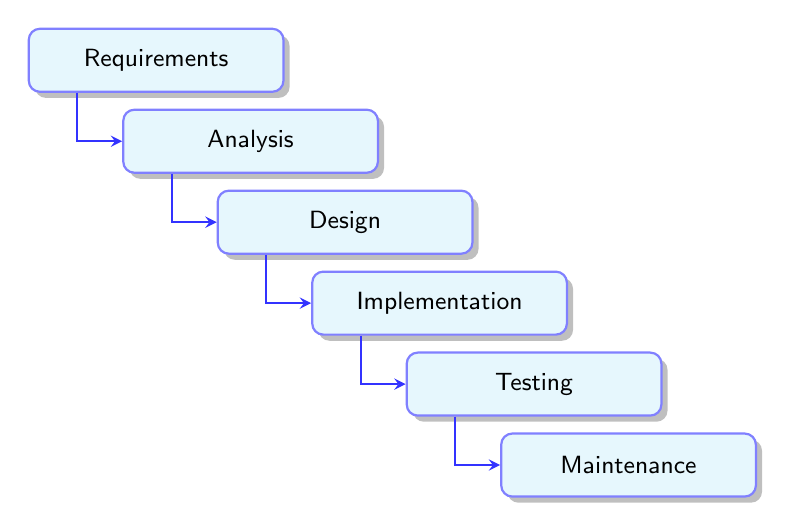
\begin{tikzpicture}[
        auto,
        every node/.style={
            rectangle, rounded corners, draw=blue!50, fill=cyan!10, thick,
            text width=3cm, align=center, font=\small, drop shadow, minimum height=0.8cm
        },
        arrow/.style={->, >=stealth, thick, color=blue!80}
    ]
        % Cascading nodes
        \node (req) {Requirements};
        \node (ana) [below=0.2cm of req, xshift=1.2cm] {Analysis};
        \node (des) [below=0.2cm of ana, xshift=1.2cm] {Design};
        \node (imp) [below=0.2cm of des, xshift=1.2cm] {Implementation};
        \node (tst) [below=0.2cm of imp, xshift=1.2cm] {Testing};
        \node (mnt) [below=0.2cm of tst, xshift=1.2cm] {Maintenance};

        % Connectors
        \draw[arrow] ([xshift=-1cm]req.south) |- (ana.west);
        \draw[arrow] ([xshift=-1cm]ana.south) |- (des.west);
        \draw[arrow] ([xshift=-1cm]des.south) |- (imp.west);
        \draw[arrow] ([xshift=-1cm]imp.south) |- (tst.west);
        \draw[arrow] ([xshift=-1cm]tst.south) |- (mnt.west);

    \end{tikzpicture}

    \small First formal Waterfall model is introduced in the 1970s. Emphasises a linear and sequential approach to software development.
\end{frame}

\begin{frame}
\frametitle{Waterfall Model}
\footnotesize
    \begin{block}{Qualities}
        \begin{itemize}
            \item Sequential design process: easy to understand and manage.
            \item Each phase must be completed before the next begins: easy to organise and coordinate.
            \item Documentation-centric: suitable for projects with well-defined requirements.
        \end{itemize}
    \end{block}

    \begin{alertblock}{Limitations}
        \begin{itemize}
            \item Inflexible to changes: not ideal for projects with evolving requirements.
            \item Late testing phase: issues may be discovered late in the process.
            \item Not suitable for complex or long-term projects: lacks iterative feedback.
        \end{itemize}
    \end{alertblock}
\end{frame}

% V-Model diagram
\begin{frame}[fragile]
    \frametitle{The V-Model}
    \centering
    \resizebox{0.95\textwidth}{!}{% Resize to fit
    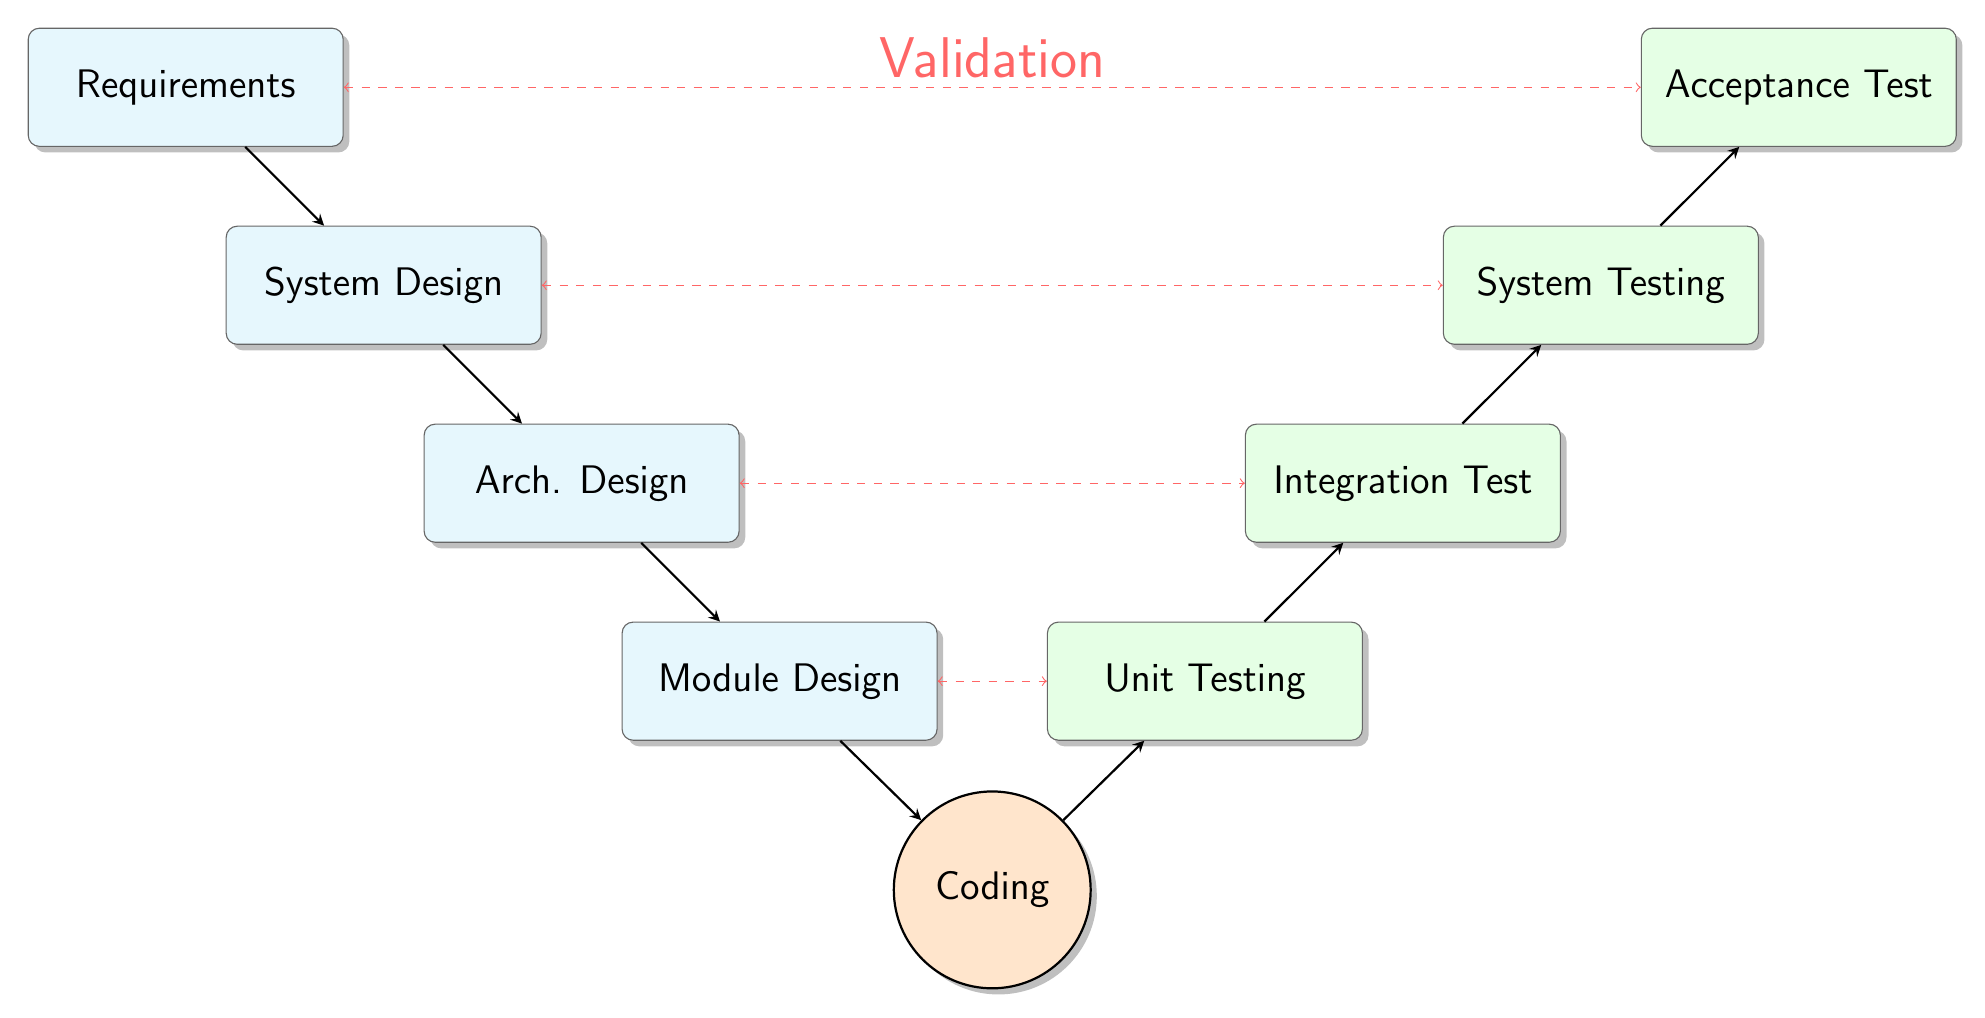
\begin{tikzpicture}[
        node distance=1.5cm,
        phase/.style={
            rectangle, draw=black!60, fill=cyan!10, rounded corners, 
            minimum width=4cm, minimum height=1.5cm, align=center, drop shadow, font=\Large
        },
        val/.style={
            rectangle, draw=black!60, fill=green!10, rounded corners, 
            minimum width=4cm, minimum height=1.5cm, align=center, drop shadow, font=\Large
        },
        arrow/.style={->, >=stealth, thick}
    ]
        % Left side
        \node[phase] (req) {Requirements};
        \node[phase, below right=1cm and -1.5cm of req] (sys) {System Design};
        \node[phase, below right=1cm and -1.5cm of sys] (arch) {Arch. Design};
        \node[phase, below right=1cm and -1.5cm of arch] (mod) {Module Design};
        
        % Bottom
        \node[circle, draw, fill=orange!20, thick, below right=1cm and -0.2cm of mod, drop shadow, minimum size=2.5cm, font=\Large] (code) {Coding};
        
        % Right side
        \node[val, above right=1cm and -0.2cm of code] (unit) {Unit Testing};
        \node[val, above right=1cm and -1.5cm of unit] (int) {Integration Test};
        \node[val, above right=1cm and -1.5cm of int] (syst) {System Testing};
        \node[val, above right=1cm and -1.5cm of syst] (acc) {Acceptance Test};

        % Flow arrows
        \draw[arrow] (req) -- (sys);
        \draw[arrow] (sys) -- (arch);
        \draw[arrow] (arch) -- (mod);
        \draw[arrow] (mod) -- (code);
        
        \draw[arrow] (code) -- (unit);
        \draw[arrow] (unit) -- (int);
        \draw[arrow] (int) -- (syst);
        \draw[arrow] (syst) -- (acc);

        % Validation lines
        \draw[dashed, <->, red!60] (req) -- (acc) node[midway, above, font=\huge] {Validation};
        \draw[dashed, <->, red!60] (sys) -- (syst);
        \draw[dashed, <->, red!60] (arch) -- (int);
        \draw[dashed, <->, red!60] (mod) -- (unit);

    \end{tikzpicture}
    }

    \small Introduced in the 1980s as an extension of the Waterfall model. Emphasises verification and validation at each stage of development.
\end{frame}
\begin{frame}
\frametitle{The V-Model}
\footnotesize
    \begin{block}{Qualities}
        \begin{itemize}
            \item Focus on testing \& quality: each development phase has a corresponding testing phase. \textit{Solves waterfall's late testing issue.}
            \item Sequential and linear phases: easy to organise and coordinate.
            \item Well suited for projects with clearly defined requirements.
        \end{itemize}
    \end{block}

    \begin{alertblock}{Limitations}
        \begin{itemize}
            \item Inflexible to changes: not ideal for projects with evolving requirements. 
            \item Assumes requirements are well understood upfront.
            \item Not suitable for complex or long-term projects: lacks iterative feedback.
        \end{itemize}
    \end{alertblock}
\end{frame}

% Incremental
\begin{frame}[fragile]
    \frametitle{Incremental Model}
    \centering
    \resizebox{0.95\textwidth}{!}{
    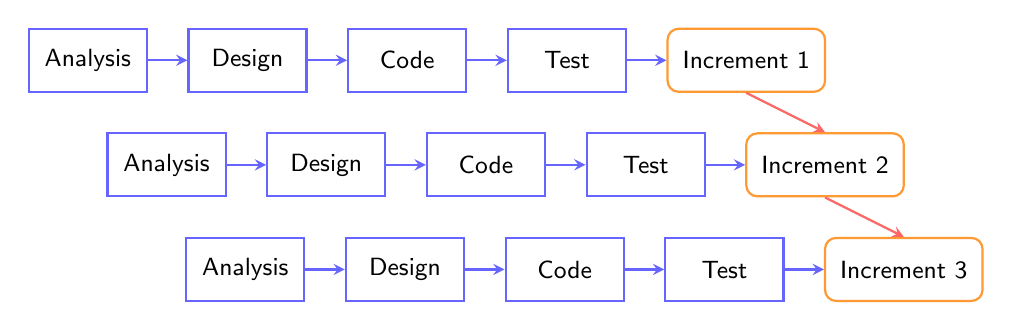
\begin{tikzpicture}[
        node distance=0.5cm,
        phase/.style={rectangle, draw=blue!60, fill=white, thick, minimum width=1.5cm, minimum height=0.8cm, align=center, font=\small},
        inc/.style={rectangle, draw=orange!80, text=black, thick, rounded corners, minimum width=2cm, minimum height=0.8cm, align=center, font=\small},
        arrow/.style={->, >=stealth, thick, blue!60},
        incarrow/.style={->, >=stealth, thick, red!60}
    ]
        % Row 1
        \node[phase] (a1) {Analysis};
        \node[phase, right=of a1] (d1) {Design};
        \node[phase, right=of d1] (c1) {Code};
        \node[phase, right=of c1] (t1) {Test};
        \node[inc, right=of t1] (i1) {Increment 1};
        
        \draw[arrow] (a1) -- (d1);
        \draw[arrow] (d1) -- (c1);
        \draw[arrow] (c1) -- (t1);
        \draw[arrow] (t1) -- (i1);
        
        % Row 2
        \node[phase, below=0.5cm of a1, xshift=1cm] (a2) {Analysis};
        \node[phase, right=of a2] (d2) {Design};
        \node[phase, right=of d2] (c2) {Code};
        \node[phase, right=of c2] (t2) {Test};
        \node[inc, right=of t2] (i2) {Increment 2};
        
        \draw[arrow] (a2) -- (d2);
        \draw[arrow] (d2) -- (c2);
        \draw[arrow] (c2) -- (t2);
        \draw[arrow] (t2) -- (i2);
        
        % Row 3
        \node[phase, below=0.5cm of a2, xshift=1cm] (a3) {Analysis};
        \node[phase, right=of a3] (d3) {Design};
        \node[phase, right=of d3] (c3) {Code};
        \node[phase, right=of c3] (t3) {Test};
        \node[inc, right=of t3] (i3) {Increment 3};
        
        \draw[arrow] (a3) -- (d3);
        \draw[arrow] (d3) -- (c3);
        \draw[arrow] (c3) -- (t3);
        \draw[arrow] (t3) -- (i3);
        
        % Increment Connections
        \draw[incarrow] (i1.south) -- (i2.north);
        \draw[incarrow] (i2.south) -- (i3.north);

    \end{tikzpicture}
    }
    
    \vspace{0.5cm}
    \raggedright
    \small System is broken down into small, manageable portions. Functional software is produced early.
\end{frame}

\begin{frame}
\frametitle{Incremental Model}
\footnotesize
    \begin{block}{Qualities}
        \begin{itemize}
            \item Each increment delivers a functional part of the system: allows for early delivery of useful software. \textit{Solves waterfall's late delivery issue.}
            \item Allows for flexibility and adaptability as each increment can be adjusted based on feedback. \textit{Solves waterfall's and v-model's inflexibility issue.}
            \item Easier to manage risks by breaking down the project into smaller parts.
        \end{itemize}
    \end{block}

    \begin{alertblock}{Limitations}
        \begin{itemize}
            \item Requires careful planning and design to ensure increments integrate well.
            \item May lead to higher overall costs due to repeated phases for each increment. Hence, not suitable for very small projects where overhead may outweigh benefits.      \end{itemize}
    \end{alertblock}
\end{frame}

% Spiral
\begin{frame}[fragile]
    \frametitle{Spiral Model}
    \centering
    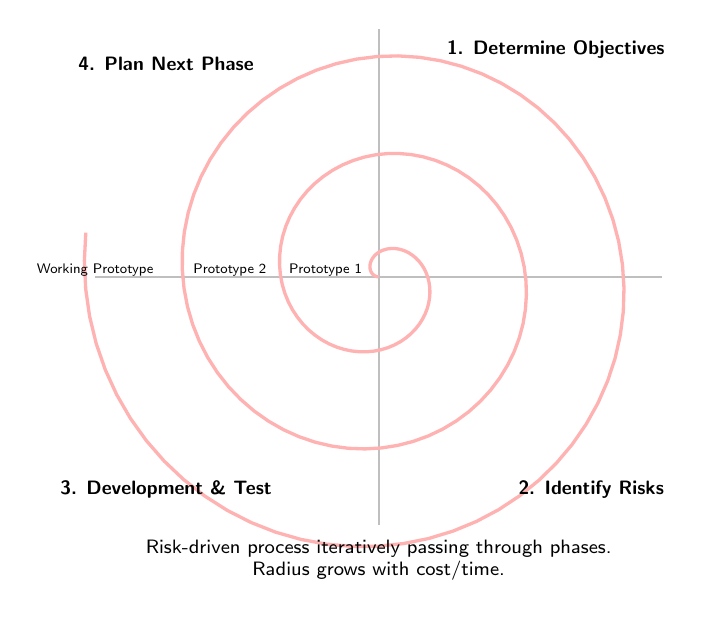
\begin{tikzpicture}[scale=0.9, font=\scriptsize, >=stealth]
        % Axes
        \draw [thick, gray!50] (-4,0) -- (4,0);
        \draw [thick, gray!50] (0,-3.5) -- (0,3.5);
        
        % Spiral
        \draw [red!30, very thick, domain=0:19, samples=200] plot ({-\x r}: {-0.22*\x});
        
        \node at (-0.75, 0.1) {\tiny Prototype 1};
        \node at (-2.1, 0.1) {\tiny Prototype 2};
        \node at (-4.0, 0.1) {\tiny Working Prototype};

        % Quadrant Labels
        \node at (2.5, 3.2) {\textbf{1. Determine Objectives}};
        \node at (3, -3) {\textbf{2. Identify Risks}};
        \node at (-3, -3) {\textbf{3. Development \& Test}};
        \node at (-3, 3) {\textbf{4. Plan Next Phase}};

        % Annotation
        \node[align=center] at (0, -4) {Risk-driven process iteratively passing through phases.\\Radius grows with cost/time.};
    \end{tikzpicture}
\end{frame}

\begin{frame}
\frametitle{Spiral Model}
\footnotesize
    \begin{block}{Qualities}
        \begin{itemize}
            \item Focus on early risk identification and mitigation: suitable for high-risk projects.
            \item Allows for iterative development and refinement based on customer's feedback.
            \item Flexible and adaptable to changing requirements at various stage of development.
        \end{itemize}
    \end{block}

    \begin{alertblock}{Limitations}
        \begin{itemize}
            \item Requires careful planning and design to ensure increments integrate well.
            \item May lead to higher overall costs due to amount of risk assessments and iterations. Hence, not suitable for very small projects where overhead may outweigh benefits.      
            \item Risk assessment and management require expertise and experience.
        \end{itemize}
    \end{alertblock}
\end{frame}

% Agile Diagram
\begin{frame}[fragile]
    \frametitle{Agile Process}
    \centering
    \resizebox{0.85\textwidth}{!}{
    \centering
    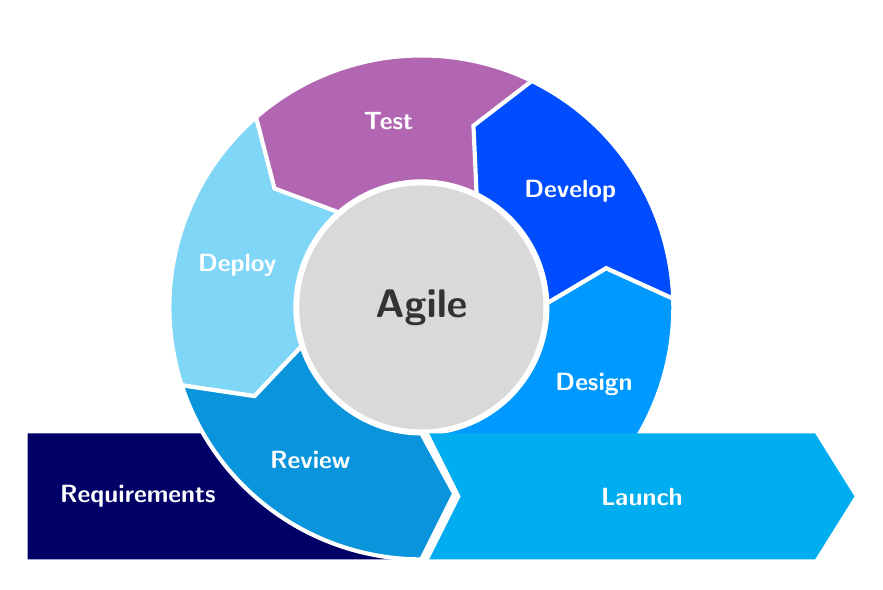
\begin{tikzpicture}[
        scale=1,
        every node/.style={font=\sffamily\bfseries\small, text=white, align=center},
        arrowsegment/.style={draw=white, line width=1.5pt}
    ]
        \def\rin{1.6}
        \def\rout{3.2}
        \def\rmid{2.4}
        
        % --- Arrows (Background Layer) ---
        % Requirements (Enters from Left, points to center-bottom)
        \fill[blue!40!black] (-5, -\rin) -- (0, -\rin) -- (0.4, -\rmid) -- (0, -\rout) -- (-5, -\rout) -- cycle;
        \node at (-3.6, -2.4) {Requirements};

        % --- Agile Cycle Segments (Clockwise) ---
        
        % 1. Test (Top): 54 to 126
        \draw[fill=violet!60, arrowsegment] (44:\rin) arc (44:136:\rin) -- (146:\rmid) -- (136:\rout) arc (136:54:\rout) -- (64:\rmid) -- cycle;
        \node at (100:\rmid) {Test};

        % 2. Deploy (Left): 126 to 198
        \draw[fill=cyan!50, arrowsegment] (131:\rin) arc (131:198:\rin) -- (208:\rmid) -- (198:\rout) arc (198:131:\rout) -- (141:\rmid) -- cycle;
        \node at (167:\rmid) {Deploy};

        % 3. Review (Bottom Left): 198 to 270
        \draw[fill=cyan!80!blue, arrowsegment] (198:\rin) arc (198:270:\rin) -- (280:\rmid) -- (270:\rout) arc (270:198:\rout) -- (208:\rmid) -- cycle;
        \node at (234:\rmid) {Review};

        % 4. Design (Bottom Right): 270 to 342
        \draw[fill=blue!40!cyan, arrowsegment] (270:\rin) arc (270:362:\rin) -- (372:\rmid) -- (362:\rout) arc (362:290:\rout) -- (300:\rmid) -- cycle;
        \node at (336:\rmid) {Design};

        % 5. Develop (Right): 342 to 414
        \draw[fill=blue!70!cyan, arrowsegment] (362:\rin) arc (362:424:\rin) -- (434:\rmid) -- (424:\rout) arc (424:362:\rout) -- (372:\rmid) -- cycle;
        \node at (398:\rmid) {Develop};

                % Launch (Exits to Right, starts from center-bottom dovetail)
        \fill[cyan] (0.1, -\rin) -- (5, -\rin) -- (5.5, -\rmid) -- (5, -\rout) -- (0.1, -\rout) -- (0.5, -\rmid) -- cycle;
        \node at (2.8, -\rmid) {Launch};

        % --- Center ---
        \node[circle, fill=gray!30, minimum size=3.1cm, text=black!80, font=\sffamily\bfseries\Large] at (0,0) {Agile};

    \end{tikzpicture}
    }
    \small Commonly described as a set of principles or a phylosophy rather than a strict methodology. Introduced in the early 2000s as a response to the limitations of traditional SDLC models.
\end{frame}

\begin{frame}
\frametitle{Agile Process}
\footnotesize
    \begin{block}{Qualities}
        \begin{itemize}
            \item Focus on customer collaboration and responsiveness to change: suitable for projects with evolving requirements.
            \item Allows for iterative development and frequent delivery of working software.
            \item Emphasises teamwork, communication, and continuous improvement.
        \end{itemize}
    \end{block}

    \begin{alertblock}{Limitations}
        \begin{itemize}
            \item Requires active customer involvement throughout the project.
            \item May lead to scope creep if not properly managed.
            \item Less emphasis on documentation may lead to challenges in knowledge transfer and maintenance.
        \end{itemize}
    \end{alertblock}
\end{frame}

\begin{frame}
    \frametitle{Next Steps}
    \begin{itemize}
        \item \textbf{This Week's Workshop:} Learning Git (Version Control).
        % \item \textbf{Reading:} Sommerville, \textit{Software Engineering 9th Edition}, Chapter 1.
        \item \textbf{Next Week:} Agile Frameworks.
    \end{itemize}
\end{frame}

\begin{frame}
    \frametitle{Q \& A}
    \begin{center}
        \Huge Any Questions?\\\vspace{0.5cm} 
        \normalsize fdelduchetto@lincoln.ac.uk
    \end{center}
\end{frame}

\end{document}